%==============================================================================
% Chapitre 72 - La rotation du projectile
%==============================================================================

\section{Introduction}

Dans un canon rayé, le projectile ne se contente pas d'accélérer
longitudinalement. Son déplacement est également accompagné d'une mise en
rotation autour de son axe.

Cette rotation constitue l'un des principaux facteurs de stabilité du
projectile pendant son vol.

\begin{aretenir}

Les rayures du canon communiquent simultanément une vitesse de translation et
une vitesse de rotation au projectile.

\end{aretenir}

\section{Principe des rayures}

Les rayures sont des rainures hélicoïdales usinées à l'intérieur du canon.

Leur géométrie impose au projectile un mouvement de rotation lors de son
déplacement.

Cette rotation débute dès les premiers millimètres parcourus dans le canon.

\begin{figure}[htbp]
\centering

\begin{tikzpicture}[scale=1]

% Canon
\draw[fill=gray!15]
(0,-0.8) rectangle (12,0.8);

% Âme
\fill[white]
(0,-0.35) rectangle (12,0.35);

% Rayures
\DrawRifling{0}{11.5}

% Projectile
\fill[blue!60]
(4,-0.30)
rectangle
(4.8,0.30);

% Flèche
\draw[-{Latex[length=3mm]},very thick,PressureColor]
(1,0.6)--(3.6,0.6);

\node[above] at (2.3,0.7)
{Déplacement};

\end{tikzpicture}

\caption{Le projectile est guidé par les rayures du canon.}
\label{fig:canon_raye}

\end{figure}

\begin{figure}[htbp]
\centering

\begin{tikzpicture}[>=Latex]

\draw[thick]
(0,0)
rectangle
(12,4);

\foreach \y in {0.5,1.5,2.5,3.5}
{
    \draw[gray]
        plot[smooth]
        coordinates{
            (0,\y)
            (3,\y+0.4)
            (6,\y)
            (9,\y-0.4)
            (12,\y)
        };
}

\draw[very thick,ProjectileColor,-{Latex[length=3mm]}]
(0,2)--(12,2);

\node[above]
at (6,4.3)
{Développement de la surface intérieure du canon};

\end{tikzpicture}

\caption{Les rayures suivent une trajectoire hélicoïdale autour de l'axe du canon.}
\label{fig:developpement_rayures}

\end{figure}

\section{Transmission du mouvement}

Lorsque le projectile s'engage dans les rayures, celles-ci exercent un effort
tangent sur son enveloppe.

Cet effort produit un couple qui met progressivement le projectile en rotation.

Le mouvement longitudinal et le mouvement de rotation sont ainsi acquis
simultanément.

\begin{figure}[htbp]
\centering

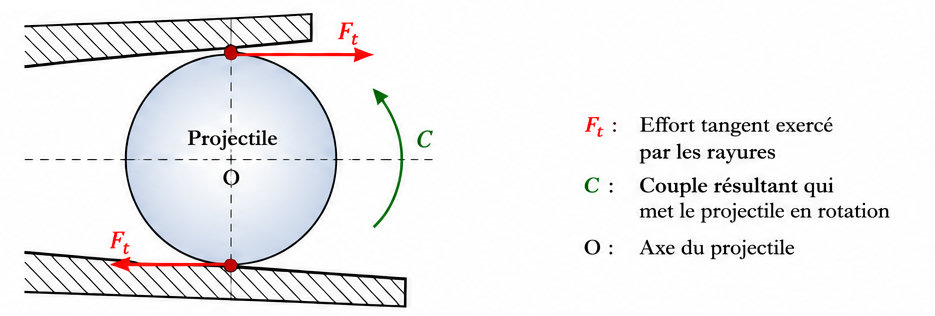
\includegraphics[width=0.7\textwidth]{figures/72.5}\\
Les efforts tangents opposés forment un couple qui provoque la rotation du projectile.
\caption{Couple exercé pas les rayures.}
\label{fig:canon_raye_I}

\end{figure}

\section{Le pas des rayures}

Le pas des rayures correspond à la longueur de canon nécessaire pour effectuer
une révolution complète.

Il constitue une caractéristique importante du canon.

Un pas plus court produit une rotation plus rapide pour une même vitesse de translation.

\begin{figure}[htbp]
\centering

\begin{tikzpicture}[>=Latex]

\draw[thick]
(0,0)
rectangle
(12,2);

\draw[very thick]
plot[smooth]
coordinates{
(0,1)
(3,1.7)
(6,1)
(9,0.3)
(12,1)
};

\draw[<->]
(0,-0.5)--(12,-0.5);

\node[below]
at (6,-0.5)
{Pas des rayures};

\end{tikzpicture}

\caption{Le pas correspond à la longueur nécessaire pour effectuer une révolution complète.}
\label{fig:pas_rayures}

\end{figure}

\begin{figure}[htbp]
\centering

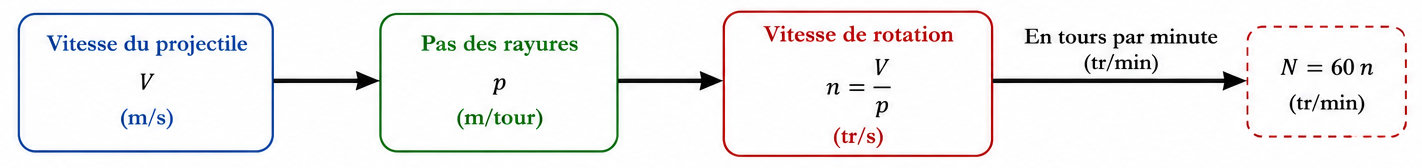
\includegraphics[width=0.85\textwidth]{figures/72.6}\\
Pour une vitesse donnée, un pas plus court produit une vitesse de rotation plus élevée.
\caption{Lien entre vitesse, pas des rayures et vitesse de rotation.}
\label{fig:canon_raye_II}

\end{figure}

\section{Vitesse de rotation}

La vitesse de rotation augmente pendant tout le parcours du projectile dans le
canon.

À la bouche, elle atteint généralement plusieurs dizaines de milliers de
tours par minute.

Cette rotation est directement liée :

\begin{itemize}
    \item à la vitesse du projectile ;
    \item au pas des rayures.
\end{itemize}

\begin{figure}[htbp]
\centering

\begin{tikzpicture}[>=Latex]

% Projectile
\fill[ProjectileColor]
(0,-0.4)
rectangle
(3,0.4);

% Translation

\draw[-{Latex[length=4mm]},very thick,PressureColor]
(-2,0.8)--(0,0.8);

\node[left]
at (-2,0.8)
{Translation};

% Rotation

\draw[very thick]
(1.5,0)
circle
(0.8);

\draw[-{Latex[length=3mm]},very thick,Part6Color]
(2.2,0)
arc
(0:270:0.8);

\node[right]
at (3.2,0)
{Rotation};

\end{tikzpicture}

\caption{Le projectile acquiert simultanément une vitesse de translation et une vitesse de rotation.}
\label{fig:translation_rotation}

\end{figure}

\begin{figure}[htbp]
\centering

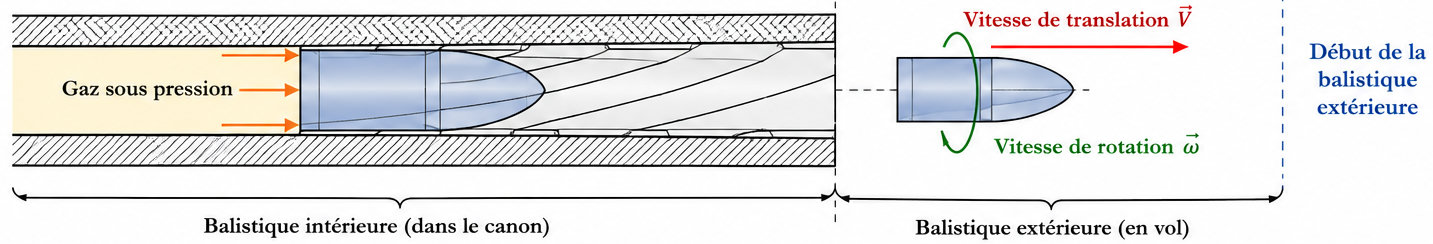
\includegraphics[width=0.95\textwidth]{figures/72.7}\\
À la sortie du canon, le projectile possède une vitesse de translation et une vitesse de rotation.
\caption{Le projectile à la sortie du canon.}
\label{fig:canon_raye_III}

\end{figure}

\section{Consommation d'énergie}

Une partie de l'énergie fournie par les gaz est utilisée pour mettre le
projectile en rotation.

Cette énergie reste toutefois faible devant celle consacrée à l'accélération
longitudinale.

\section{Influence sur la stabilité}

La rotation stabilise le projectile par effet gyroscopique.

Elle limite les variations d'orientation au cours du vol et contribue à la
précision du tir.

Cette stabilité sera étudiée plus en détail dans la partie consacrée à la
balistique extérieure.

\section{Influence du projectile}

La vitesse de rotation dépend également des caractéristiques du projectile,
notamment de sa longueur, de sa masse et de la position de son centre de
gravité.

Ces paramètres interviennent dans le choix du pas des rayures.

\section{Observation expérimentale}

La rotation peut être observée à l'aide de caméras ultra-rapides ou déduite à
partir des caractéristiques du canon et de la vitesse mesurée à la bouche.

Les marques laissées par les rayures permettent également d'étudier ce
phénomène.

\section{Modélisation en simulation}

\begin{simulation}

Les simulateurs de balistique calculent généralement la vitesse de rotation à
partir de la vitesse longitudinale du projectile et du pas des rayures.

Cette grandeur est ensuite utilisée dans les modèles de stabilité
gyroscopique développés en balistique extérieure.

\end{simulation}

\section{Vers la sortie du canon}

À la fin de son parcours dans le canon, le projectile possède simultanément :

\begin{itemize}
    \item une vitesse de translation ;
    \item une vitesse de rotation.
\end{itemize}

Ces deux composantes détermineront son comportement dès sa sortie de bouche.

\begin{formule}{Vitesse de rotation}

La vitesse de rotation est directement liée à la vitesse du projectile et au
pas des rayures.

\[
n=\frac{V}{p}
\]

où :

\begin{description}
\item[$n$] fréquence de rotation (tr/s)
\item[$V$] vitesse du projectile (m/s)
\item[$p$] pas des rayures (m/tr)
\end{description}

Pour obtenir une vitesse de rotation en tours par minute :

\[
N=60\,n
\]

\end{formule}

\section{À retenir}

\begin{aretenir}

\begin{itemize}
    \item Les rayures mettent le projectile en rotation.
    \item La rotation est acquise progressivement pendant le parcours dans le
          canon.
    \item Le pas des rayures détermine la vitesse de rotation.
    \item La rotation stabilise le projectile pendant son vol.
    \item La stabilité gyroscopique sera étudiée en balistique extérieure.
\end{itemize}

\end{aretenir}
